\documentclass[11pt]{amsart}
\usepackage{geometry}                % See geometry.pdf to learn the layout options. There are lots.
\geometry{letterpaper}                   % ... or a4paper or a5paper or ... 
%\geometry{landscape}                % Activate for for rotated page geometry
%\usepackage[parfill]{parskip}    % Activate to begin paragraphs with an empty line rather than an indent
\usepackage{graphicx}
\usepackage{amssymb}
\usepackage{epstopdf}
\DeclareGraphicsRule{.tif}{png}{.png}{`convert #1 `dirname #1`/`basename #1 .tif`.png}

\title{Brief Brainz Article}
\author{Tim and Cyrille}
%\date{}                                           % Activate to display a given date or no date


\begin{document}
\section{Introduction}
Optical ray\footnote{Source wikipedia} tracing describes a method for producing visual images constructed in 3D computer graphics environments. It works
by tracing a path from an imaginary eye through each pixel in a virtual screen. 

\begin{figure}[htbp]
\begin{center}
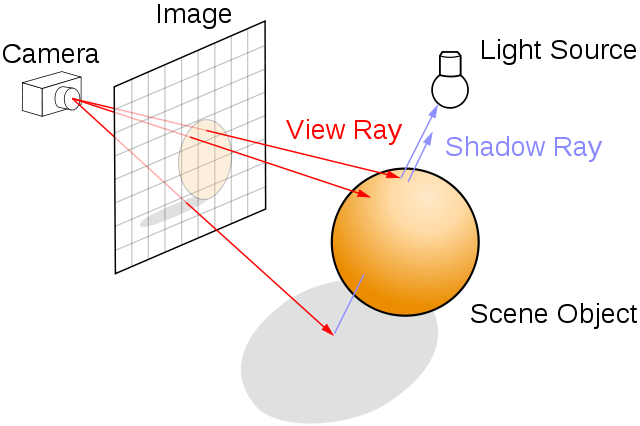
\includegraphics[scale=0.35]{640px-Ray_trace_diagram}
\caption{The ray tracing algorithm builds an image by extending rays into a scene. \label{fig1}}
\end{center}
\end{figure}

Each ray must be tested with some subset of all objects of the scenes (figure \ref{fig1}). The interactions of the paths and the scene necessitate to compute 
the new properties (in function of the characteristic of the object: e.g. absorption, reflection, refraction or fluorescence) of the ray and 
consequently modify the color of the pixel. The principles of starting the rays from the eye (named "backwards") seems counterintuitive, 
rather than into it (Light source to the screen). This backwards method is many orders of magnitude moe efficient. 
Because "forward" simulation wastes a large number of rays, because they will never reach the virtual screen.

\section{sphere example \label{SECTION_EX}}
The main work of the ray tracing method is to compute the intersection between the ray and the object. A good example, is the interaction 
between the rays and a sphere, a well know model in mathematic. Operations are performed using vectorial notation (bold font) $\mathbf{r}$,
and $\hat{\mathbf{r}} = \frac{\mathbf{r}}{|r|}$.

The equation of the sphere with center $\bf{c}$ and radius $r$ is 
\begin{eqnarray}
	||\mathbf{x}-\mathbf{c}||^2 = r^2  \label{REF0}
\end{eqnarray}
Any point on a ray  starting from the point $\bf{s}$ with direction given by $\hat{\mathbf{d}}$ can be written by 
\begin{eqnarray}
	\mathbf{x}  =  \mathbf{s} + t\mathbf{d},    \nonumber
\end{eqnarray}
Where $t$ the unknown describes the "distance" between the source ($\mathbf{s}$) and the sphere ($\mathbf{x}$).
If we substitute $\mathbf{x}$ in the equation \ref{REF0} and define $\bf{v} = s-c$, then
\begin{eqnarray}
	||\mathbf{v} + t\mathbf{d}||^2  & = & r^2  \nonumber \\ 
	\mathbf{v}^2 + t^2 \mathbf{d}^2 + 2\mathbf{v}.t\mathbf{d} & = & r^2  \nonumber \\
	t^2  + (2\mathbf{v}.\mathbf{d}t) +(\mathbf{v}^2-r^2) & = & 0 \nonumber
\end{eqnarray}
This quadratic equation is well know and has two solutions (if the descriminant is not negative)
\begin{eqnarray}
	t = - (\mathbf{v}.\mathbf{d})\pm\sqrt{(\mathbf{v}.\mathbf{d})^2-(\mathbf{v}^2 - r^2)}
\end{eqnarray}
The different solution may be represented by the following scheme.
\begin{figure}[htbp]
\begin{center}
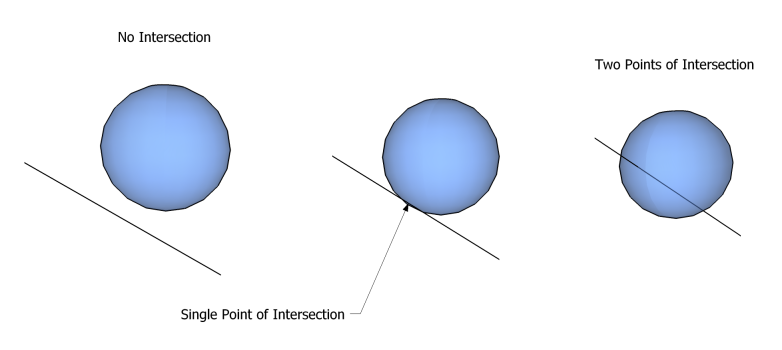
\includegraphics[scale=0.5]{Line-Sphere_Intersection_Cropped}
\caption{Intersection of the sphere with a ray. \label{fig2}}
\end{center}
\end{figure}

When the intersection has been found, the new direction of the ray must be determinate. If we consider a perfect reflective surface (figure \ref{fig3} specular reflection), the angle of the incident ray with the normal of the sphere will be the same that the angle of the reflection 

\begin{figure}[htbp]
\begin{center}
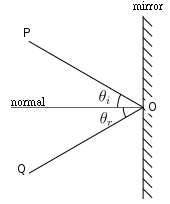
\includegraphics[scale=0.5]{170px-Reflection_angles}
\caption{Specular reflection \label{fig3}}
\end{center}
\end{figure}

The normal of the sphere is given by

\begin{eqnarray}
\mathbf{n} = \frac{\mathbf{y} - \mathbf{c}}{||\mathbf{y} - \mathbf{c}||} \nonumber
\end{eqnarray}

where $\mathbf{y}  =  \mathbf{s} + t\mathbf{d}$ is the intersection found before. The new reflection direction $\mathbf{r}$ with the respect of the normal of the sphere is 

\begin{eqnarray}
\mathbf{r} = \mathbf{d} - 2(\mathbf{n}.\mathbf{d})\mathbf{n} \nonumber
\end{eqnarray}

Thus the reflected ray has the new equation and direction ($\mathbf{r}$): $\mathbf{x}  =  \mathbf{y} + u\mathbf{r}$.

The last step consist to evaluate the color of the pixel. If a ray is assimilated to a "red" single photon, the energy of the photon
is given by $E = \frac{hc}{\lambda}$, $h$ is the Planck constant, $c$ the speed of light in vacuum and $\lambda$ the photon wavelength 
(780 $nm$ for the red). During the interaction with the material, physicochemical reactions can be imagined and modify the wavelength of
the photon (the ray) and consequently the color of the pixel. 

At the end multiples ray per pixel can occurs, the combinaison with all interactions will create a nice picture. 
To conclude, as  it is described the problem, ray tracing is a very good algorithm for parallel computing because each ray does not interact each other,
consequently they can be computed independently using all standards technologies (SIMD, thread, MPI, {\it etc ...})

\section{Brayns workflow}

The Brayns  (BraynsView) software can perform visualisation of the morphology of the Brain. The visualisation is performed using ray tracing technic with the help
the external library Ospray developed by Intel. Ospray is an open source, scalable (multiscale MPI and threading) ray  tracing library engine for CPU only. The library
is built over the embree library (also intel), that provides primitives for ray tracing. The library has the particularity to be built over ISPC (llvm frontend) compiler that generates 
tuned SIMD kernels.  

Personal consideration: the HPC team has a good experience of vectorization, the approach  of using a DSL associated to a specific compiler (ISPC) allows better possible optimisation.
In fact in a normal DSL (like cyme) every node of the build DAG is associated to a final intriniscs SIMD wrapper that call internally an inline ASM block. Consequently, the compiler
can not make optimization like merging instruction, or remove duplicate instructions.  As ISPC is related to the LLVM backend, I suppose ISPC  uses specific tools of LLVM. The disadvantage is less flexibility.

\begin{center}
\begin{figure}[h]
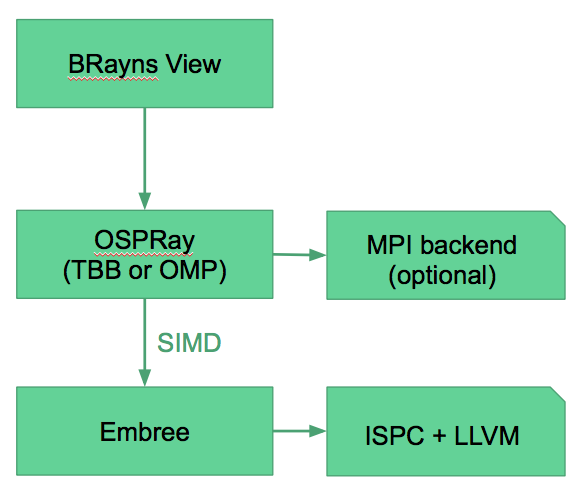
\includegraphics[scale=0.27]{workflowbrayns}
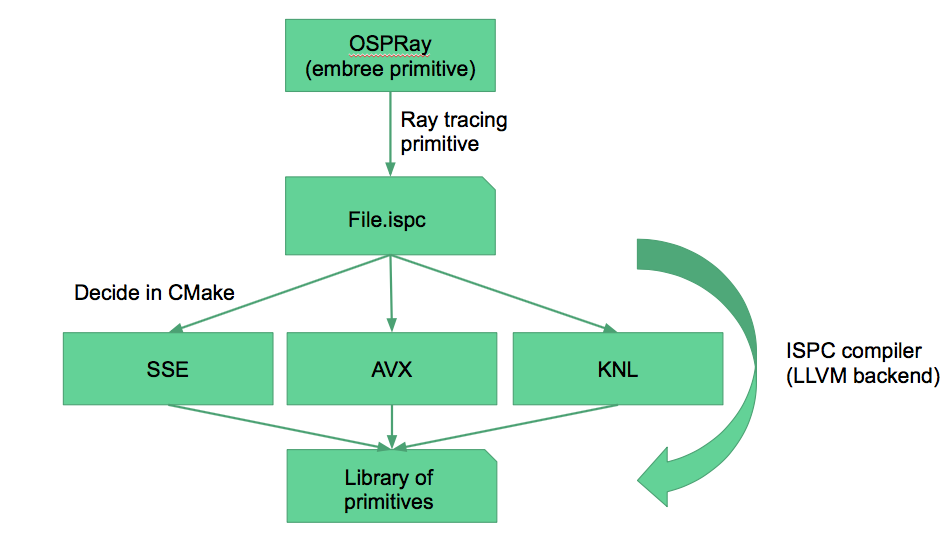
\includegraphics[scale=0.27]{SIMD}
\caption{Global workflow of Brayns  and Ospray \label{workflow}}
\end{figure}
\end{center}

The code has been developed independently of the ray tracing library, Ospray could be changed by any alternative like the Nvidia 
library Optics. The global workflow of the library is presented in the figure \ref{workflow}.

\section{Ospray compilation and options}

Ospray provides freedom for the user, MPI distribution, threading  (OMP or TBB) and SIMD agnostic. Ospray has in own copy of embree. We summurize the options and the corresponding option
of compilation of the library in the following table:

\begin{table}[h]
\caption{CMake options of the Ospray  and Embree libraries}
\begin{center}
\begin{tabular}{c c}
CMake Flag                                                                   & value \\
\hline
 -DOSPRAY\_BUILD\_MPI\_DEVICE          &  ON \\
 -DOSPRAY\_TASKING\_SYSTEM  & TBB (default) /  OpenMP    \\
 -DOSPRAY\_BUILD\_ISA                   & ALL (default) /SSE/AVX/AVX2 \\
\hline
\end{tabular}
\end{center}
\label{default}
\end{table}%

User must set up running time option during the run specially to indicate a parallel execution {\tt--osp:mpi} , {\tt--osp:numthreads <\#numthreads>}  or set up the number of threads.

\section{BRayns and Ospray performance, preliminary work}

A simple profiling (hotspots with vtune) offers already a good point of view of the performance and the bottle neck of the application.  More than 90\% of the time is spent into
the ray/object intersection section (\ref{SECTION_EX}) detection, using the AVX backend of embree.

\begin{table}[h]
\caption{Vtune 16 threads, viz cluster, on a run of 12 [s] \label{PROF}}
\begin{center}
\begin{tabular}{l c }
functions &  elapse time [s] \\
\hline
embree::avx::BVH4Intersector8Chunk & 10.277 \\
\,\,\,-ExtendedCylinders\_intersect   &  6.026  \\
\,\,\,-ExtendedSpheres\_intersect & 4.235 \\
\hline
\end{tabular}
\end{center}
\label{default}
\end{table}%




\end{document} 